\documentclass{article}

\usepackage{préambule}
\usepackage[margin=0.5cm]{geometry}
\usetikzlibrary{calc}


\begin{document}

\begin{center}
	\pgfmathsetmacro\MaScaleInv{0.35}
	\pgfmathsetmacro\MaScale{1 / \MaScaleInv}
	\newcommand{\LargeurImage}{16}
	\begin{tikzpicture}[scale=\MaScaleInv]
		\node [anchor=south west] at ($\MaScale*(-0.12,-0.12)$) {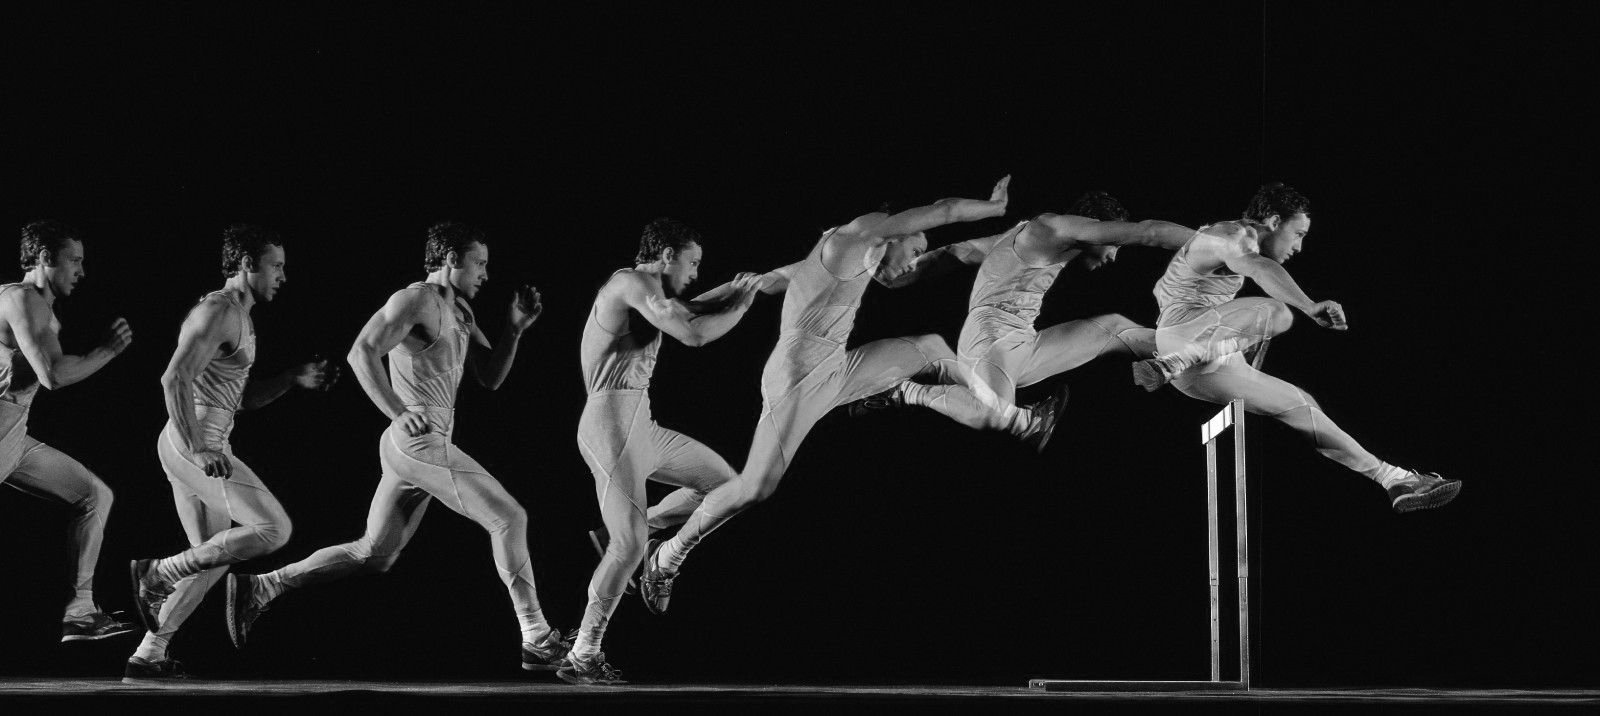
\includegraphics[width=\LargeurImage cm]{images/chronophotographie saut d'obstacle.jpeg}};
		\draw[white,ultra thin] (0,0) grid ++($\MaScale*(\LargeurImage,\LargeurImage * 716 / 1600)$);

		\ifdefined\makeCorrection
			\coordinate (P0) at (0.82,4.43);
			\coordinate (P1) at (2.87,4.38);
			\coordinate (P2) at (4.88,4.35);
			\coordinate (P3) at (7,4.37);
			\coordinate (P4) at (9.17,4.48);
			\coordinate (P5) at (11.13,4.55);
			\coordinate (P6) at (13,4.65);
			\foreach \p in {P0,P1,P2,P3,P4,P5,P6} {
					\node[red] at ($\MaScale*(\p)$) {×};
					\node[red,below left] at ($\MaScale*(\p)$) {$\p$};
				}
		\fi
	\end{tikzpicture}
\end{center}

\begin{multicols}{3}
	\begin{itemize}
		\item Le point en bas à gauche a pour coordonnées $(0 ; 0)$.
		\item Il y a $20$ cm par carreau.
		\item L'intervalle entre chaque photographie est de $0,2$ secondes.
	\end{itemize}
\end{multicols}

\vfill
\hrule

\begin{center}
	\pgfmathsetmacro\MaScaleInv{0.45}
	\pgfmathsetmacro\MaScale{1 / \MaScaleInv}
	\newcommand{\LargeurImage}{16}
	\begin{tikzpicture}[scale=\MaScaleInv]
		\node[anchor=south west] at ($\MaScale*(-0.12,-0.12)$) {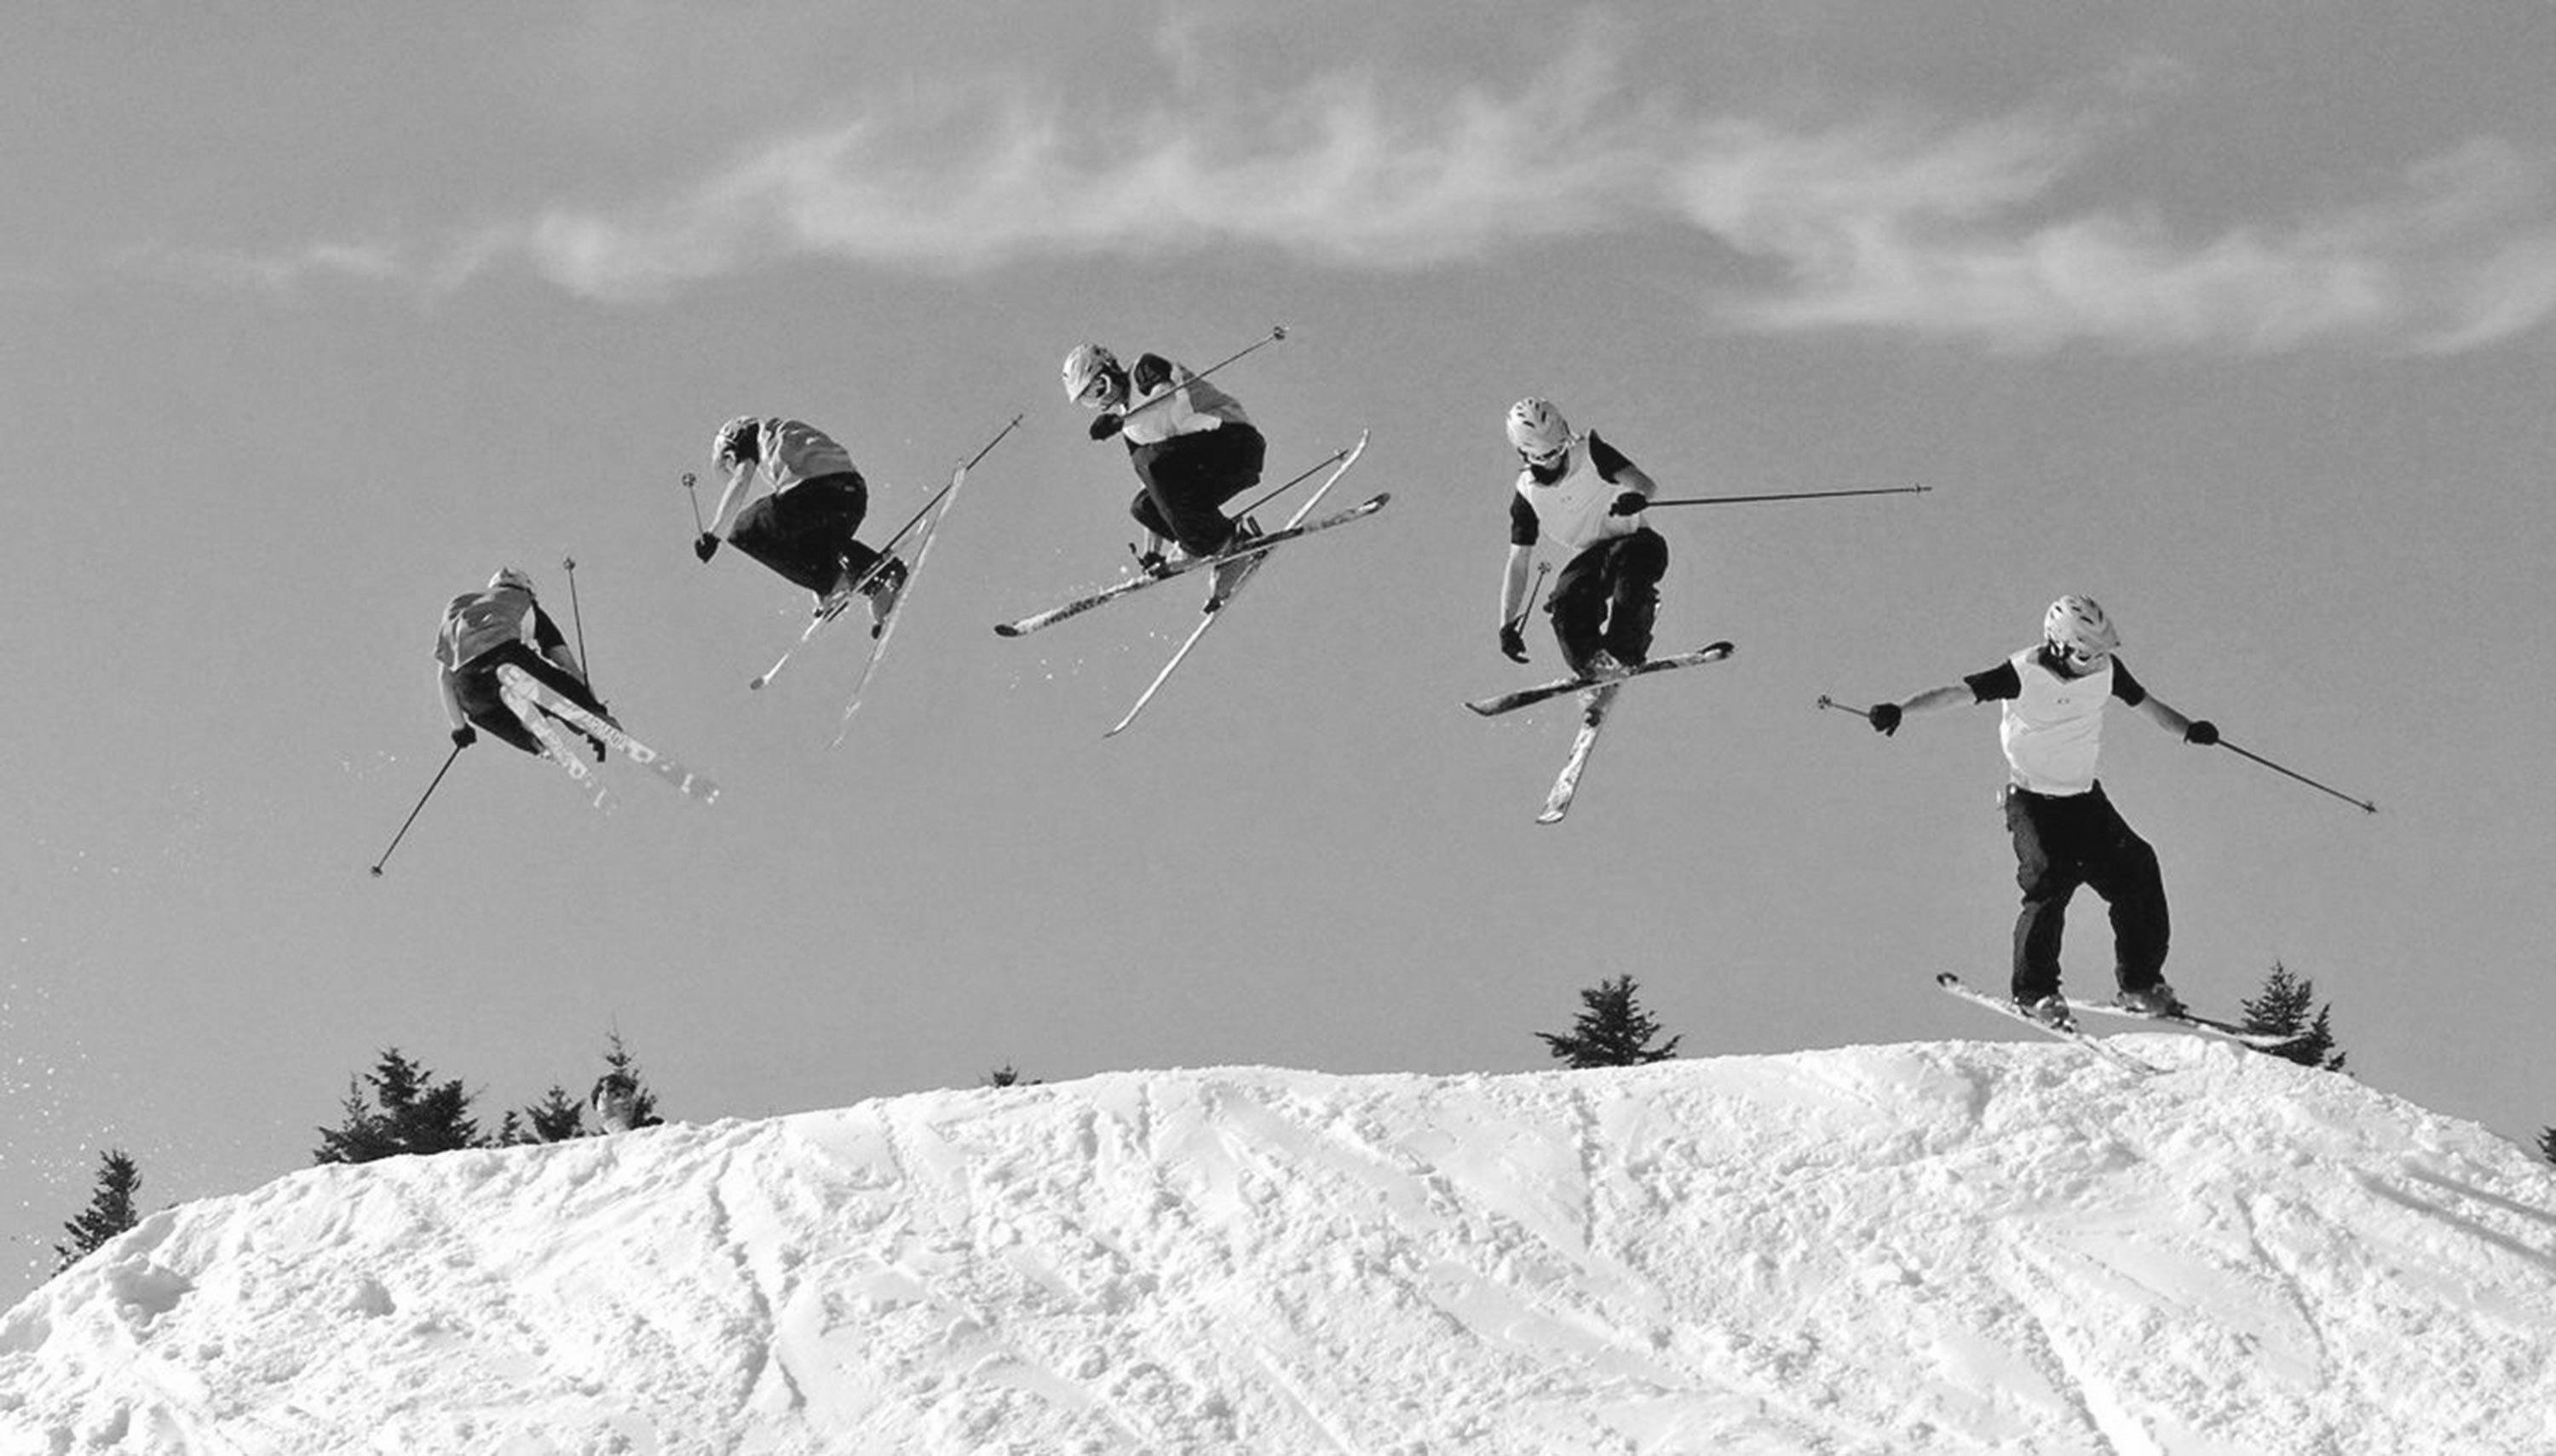
\includegraphics[width=\LargeurImage cm]{images/chronophotographie skieur.jpeg}};
		\draw[black,ultra thin] (0,0) grid ++($\MaScale*(\LargeurImage,\LargeurImage / 3000 * 1709)$);
		\ifdefined\makeCorrection
			\coordinate (P0) at (3.55,5.58);
			\coordinate (P1) at (4.32,6.12);
			\foreach \p in {P0,P1} {
					\node[red] at ($\MaScale*(\p)$) {×};
					\node[red,below left] at ($\MaScale*(\p)$) {$\p$};
				}
		\fi
	\end{tikzpicture}
\end{center}

\begin{multicols}{3}
	\begin{itemize}
		\item Le point en bas à gauche a pour coordonnées $(0 ; 0)$.
		\item Il y a $30$ cm par carreau.
		\item L'intervalle entre chaque photographie est de $0,2$ secondes.
	\end{itemize}
\end{multicols}

\vfill

\end{document}